\documentclass[tikz,border=12pt]{standalone}
\usepackage{amsmath,amssymb}
\usetikzlibrary{calc,arrows.meta}

\begin{document}
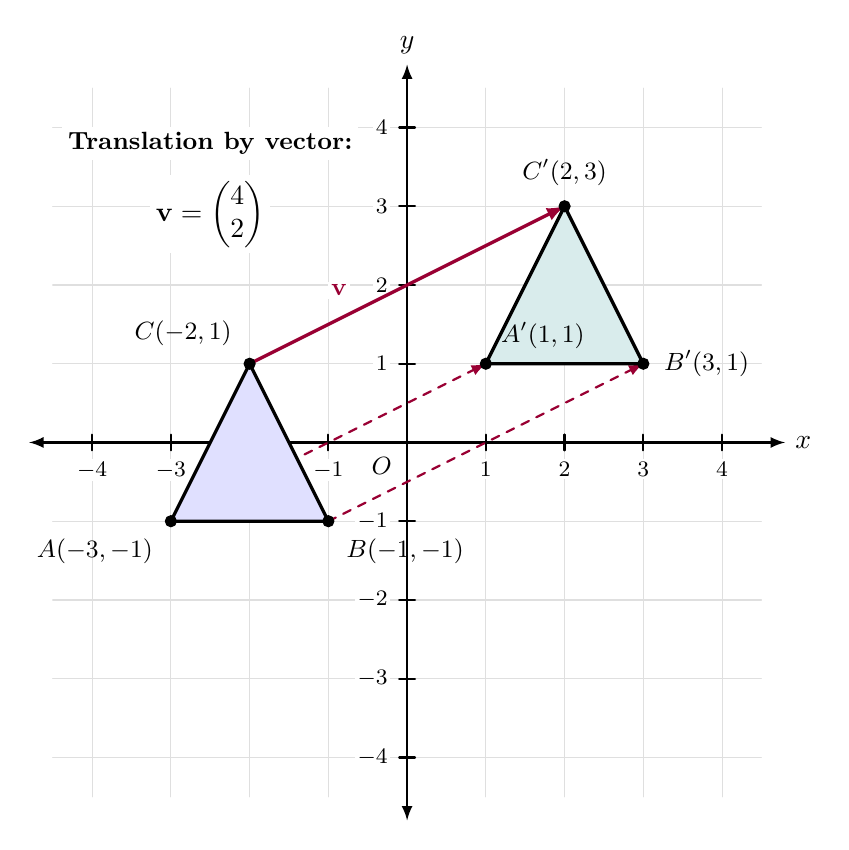
\begin{tikzpicture}[>=latex, line cap=round, line join=round]
  % Grid
  \draw[step=1cm, gray!25, thin] (-4.5, -4.5) grid (4.5, 4.5);

  % Axes
  \draw[thick, <->] (-4.8, 0) -- (4.8, 0) node[right, font=\normalsize] {$x$};
  \draw[thick, <->] (0, -4.8) -- (0, 4.8) node[above, font=\normalsize] {$y$};

  % Origin
  \node[below left=2pt, font=\small] at (0, 0) {$O$};

  % Integer ticks with opaque backgrounds to prevent line collision
  \foreach \x in {-4,-3,-2,-1,1,2,3,4} {
    \draw[thick] (\x, 0.1) -- (\x, -0.1);
    \node[below=3pt, font=\footnotesize, fill=white, inner sep=1pt] at (\x, -0.1) {$\x$};
  }
  \foreach \y in {-4,-3,-2,-1,1,2,3,4} {
    \draw[thick] (0.1, \y) -- (-0.1, \y);
    \node[left=3pt, font=\footnotesize, fill=white, inner sep=1pt] at (-0.1, \y) {$\y$};
  }

  % Object triangle ABC (Quadrant III)
  \coordinate (A) at (-3, -1);
  \coordinate (B) at (-1, -1);
  \coordinate (C) at (-2, 1);

  % Image triangle A'B'C' translated by vector (4, 2) (Quadrant I)
  \coordinate (A1) at (1, 1);
  \coordinate (B1) at (3, 1);
  \coordinate (C1) at (2, 3);

  % Translation displacement vectors
  \draw[very thick, ->, purple!80!black] (C) -- (C1) node[pos=0.35, above left=3pt, font=\small\bfseries, fill=white, inner sep=1pt] {$\mathbf{v}$};
  \draw[thick, dashed, ->, purple!80!black] (A) -- (A1);
  \draw[thick, dashed, ->, purple!80!black] (B) -- (B1);

  % Object triangle ABC
  \draw[very thick, fill=blue!12] (A) -- (B) -- (C) -- cycle;
  \filldraw[black] (A) circle (2pt) node[below left=3pt, font=\small\bfseries] {$A(-3,-1)$};
  \filldraw[black] (B) circle (2pt) node[below right=3pt, font=\small\bfseries] {$B(-1,-1)$};
  \filldraw[black] (C) circle (2pt) node[above left=3pt, font=\small\bfseries] {$C(-2,1)$};

  % Image triangle A'B'C'
  \draw[very thick, fill=teal!15] (A1) -- (B1) -- (C1) -- cycle;
  \filldraw[black] (A1) circle (2pt);
  \node[above right=2pt, font=\small\bfseries] at (A1) {$A'(1,1)$};
  \filldraw[black] (B1) circle (2pt) node[right=4pt, font=\small\bfseries] {$B'(3,1)$};
  \filldraw[black] (C1) circle (2pt) node[above=4pt, font=\small\bfseries] {$C'(2,3)$};

  % Translation Vector Rule Annotation in Quadrant II
  \node[font=\small\bfseries, fill=white, inner sep=2pt] at (-2.5, 3.8) {Translation by vector:};
  \node[font=\normalsize, fill=white, inner sep=2pt] at (-2.5, 2.9) {$\mathbf{v} = \begin{pmatrix} 4 \\ 2 \end{pmatrix}$};

\end{tikzpicture}
\end{document}
